% ============================================================
% The First Pass: A Complete Worked Example Through the
% Generative-Collapse Spine
%
% Compile: pdflatex → bibtex → pdflatex → pdflatex
% ============================================================

\documentclass[
  aps,
  prd,
  twocolumn,
  superscriptaddress,
  nofootinbib,
  floatfix
]{revtex4-2}

% ── packages ──
\usepackage{amsmath,amssymb,amsthm,mathtools}
\usepackage{graphicx}
\usepackage{xcolor}
\definecolor{linkblue}{HTML}{337799}
\usepackage[colorlinks=true,linkcolor=linkblue,citecolor=linkblue,urlcolor=linkblue]{hyperref}
\usepackage{bm}
\usepackage{booktabs}
\usepackage{multirow}
\usepackage{xfrac}
\usepackage{enumitem}
\usepackage{array}
\usepackage{fancyvrb}
\usepackage{caption}
\usepackage{tikz}
\usetikzlibrary{positioning, arrows.meta}
\usepackage[most]{tcolorbox}
\newcolumntype{P}[1]{>{\raggedright\arraybackslash}p{#1}}

% ── theorem environments ──
\newtheorem*{axiom}{Axiom}
\newtheorem{theorem}{Theorem}
\newtheorem{definition}[theorem]{Definition}
\newtheorem{lemma}[theorem]{Lemma}
\newtheorem{corollary}[theorem]{Corollary}
\newtheorem{proposition}[theorem]{Proposition}
\newtheorem{identity}[theorem]{Identity}
\newtheorem{remark}{Remark}

% ── UMCP macros ──
\newcommand{\tR}{\tau_{\!R}}
\newcommand{\tRS}{\tau_{\!R}^{*}}
\newcommand{\Gam}{\Gamma}
\newcommand{\eps}{\varepsilon}
\newcommand{\IR}{\infty_{\mathrm{rec}}}
\newcommand{\tolseam}{\mathrm{tol}_{\mathrm{seam}}}
\newcommand{\dd}{\mathrm{d}}
\newcommand{\Res}{\mathrm{Res}}
\newcommand{\beq}{\begin{equation}}
\newcommand{\eeq}{\end{equation}}
\newcommand{\INF}{\texttt{INF\_REC}}
\newcommand{\regime}[1]{\textrm{\upshape\scshape#1}}
\newcommand{\conform}{\regime{conformant}}
\newcommand{\nonconform}{\regime{nonconformant}}
\newcommand{\neval}{\regime{non-evaluable}}
\newcommand{\tvec}{\mathbf{c}}
\newcommand{\wvec}{\mathbf{w}}
\newcommand{\IC}{\mathrm{IC}}
\newcommand{\gF}{g_{\!F}}
\newcommand{\RunID}{\mathrm{RunID}}

\begin{document}

% ============================================================
% TITLE
% ============================================================
\title{The First Pass: A Complete Worked Example Through the
Generative-Collapse Spine}

\author{Clement Paulus}
\email{clementpaulus9@gmail.com}
\affiliation{UMCP / GCD / RCFT Canon}
\affiliation{UMCP Reference Implementation, GitHub}

\date{\today}

\begin{abstract}
This paper is the shortest complete route through the
Generative Collapse Dynamics (GCD) validation spine.  We trace a
single measurement---three voltage readings at 99\% fidelity---from
Axiom-0 (``Collapse is generative; only what returns is real'')
through every stop of the Universal Measurement Contract Protocol
(UMCP): frozen contract, bounded embedding, kernel computation,
integrity ledger, regime classification, and three-valued verdict.
Every number is exact, every identity is verified to machine
precision, and every step is reproducible from the open-source
reference implementation.  A heterogeneous counterexample exposes
geometric slaughter---the mechanism by which a single degraded
channel destroys multiplicative coherence while the arithmetic mean
appears healthy.  The paper requires no prior knowledge of the
framework: a reader who has followed one complete pass can navigate
any domain closure, any theorem, and any extension of the system.
\end{abstract}

\maketitle

% ============================================================
\section{Introduction}\label{sec:intro}
% ============================================================

The Generative Collapse Dynamics (GCD) framework and its operational
arm, the Universal Measurement Contract Protocol
(UMCP)~\cite{paulus2025umcp,paulus2025physicscoherence}, have been
validated across 23 domain
closures~\cite{umcpmetadatarepo}---from particle
physics~\cite{paulus2025physicscoherence} to consciousness
coherence---with 20{,}221 automated tests, 47~lemmas, and
44~structural identities verified to machine precision.  Yet no
single document has traced one complete object through every layer
of the system: from the axiom through the frozen contract, embedding,
kernel computation, ledger reconciliation, regime classification,
casepack packaging, and operational execution---all with exact numbers.

This paper provides that trace.  The object is deliberately
minimal: three identical voltage readings.  This choice is
architectural, not pedagogical laziness.  The validation spine is
\emph{invariant} across domains: the same frozen contract, kernel,
ledger, regime gates, and verdict logic apply whether the trace
vector carries three voltages or thirty-one Standard Model
particles.  Only the Tier-2 closure changes---the mapping from raw
observables to the unit interval.  A reader who has verified the
spine for the simplest case can navigate any domain closure by
understanding only the channel selection, never the protocol itself.
A \emph{closure} is precisely this mapping layer: it selects which
real-world quantities become the trace vector's channels and weights,
but does not alter the kernel or the protocol that evaluates them.

\subsection{Scope and structure}

We present twelve stops, organized into the five stages of the
fixed discourse spine:
\begin{enumerate}[leftmargin=*]
\item \textbf{Contract} (Stops~1--2): The axiom is stated; the
  contract is frozen.
\item \textbf{Canon} (Stops~3--5): Channels are chosen, the trace
  is bounded, and the kernel is computed.
\item \textbf{Closures} (Stop~6): Thresholds are published; the
  ledger is debited and credited.
\item \textbf{Integrity Ledger} (Stop~7): The seam residual is
  checked; the regime is classified.
\item \textbf{Stance} (Stops~8--12): The verdict is derived;
  the result is packaged, executed, rendered, and read back into
  ordinary language.
\end{enumerate}

Figure~\ref{fig:spine} maps the twelve stops onto the five spine
stages visually.

\begin{center}
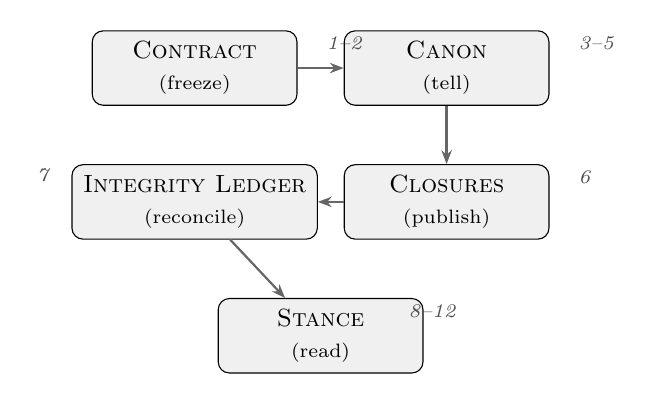
\begin{tikzpicture}[
  font=\small,
  stage/.style={draw, rectangle, rounded corners=4pt, inner sep=4pt,
    minimum width=2.6cm, minimum height=0.9cm, align=center,
    fill=black!6, font=\scshape\small},
  stop/.style={font=\scriptsize, text=black!70, align=left},
  arr/.style={-{Stealth[length=5pt]}, thick, black!60},
]
  % Row 1: Contract and Canon
  \node[stage] (contract) at (0,0) {Contract \\ \normalfont\scriptsize (freeze)};
  \node[stage] (canon) at (3.2,0) {Canon \\ \normalfont\scriptsize (tell)};

  % Row 2: Closures (centered, staggered down)
  \node[stage] (closures) at (3.2,-1.7) {Closures \\ \normalfont\scriptsize (publish)};

  % Row 3: Ledger and Stance
  \node[stage] (ledger) at (0,-1.7) {Integrity Ledger \\ \normalfont\scriptsize (reconcile)};
  \node[stage] (stance) at (1.6,-3.4) {Stance \\ \normalfont\scriptsize (read)};

  % Arrows: zigzag path
  \draw[arr] (contract) -- (canon);
  \draw[arr] (canon) -- (closures);
  \draw[arr] (closures) -- (ledger);
  \draw[arr] (ledger) -- (stance);

  % Stop annotations (right side of each node)
  \node[stop, anchor=west] at (contract.east)
    [xshift=7pt, yshift=9pt] {\textit{1--2}};
  \node[stop, anchor=west] at (canon.east)
    [xshift=7pt, yshift=9pt] {\textit{3--5}};
  \node[stop, anchor=west] at (closures.east)
    [xshift=7pt, yshift=9pt] {\textit{6}};
  \node[stop, anchor=west] at (ledger.west)
    [xshift=-16pt, yshift=9pt] {\textit{7}};
  \node[stop, anchor=east] at (stance.east)
    [xshift=16pt, yshift=9pt] {\textit{8--12}};
\end{tikzpicture}

\vspace{0.4cm}
{\footnotesize\setlength{\tabcolsep}{2pt}%
\begin{tabular}{@{}c@{\;}l@{\;\;}l@{\;\;}l@{}}
  \toprule
  \textbf{Stop} & \textbf{What happens} & \textbf{Stage} & \textbf{Tier} \\
  \midrule
  1 & Axiom declared    & \multirow{2}{*}{\textsc{Contract}} & 1 \\
  2 & Params frozen     & & 0 \\
  \midrule
  3 & Channels chosen   & \multirow{3}{*}{\textsc{Canon}} & 2 \\
  4 & Trace bounded     & & 0 \\
  5 & Kernel computed   & & $1\!\leftarrow\!0$ \\
  \midrule
  6 & Ledger debited    & \textsc{Closures} & 0 \\
  \midrule
  7 & Regime classified & \textsc{Ledger} & 0 \\
  \midrule
  8 & Casepack built    & \multirow{5}{*}{\textsc{Stance}} & 0 \\
  9 & CLI executed      & & 0 \\
  10 & API called       & & 0 \\
  11 & Latin rendered   & & 2 \\
  12 & Ordinary reading & & 2 \\
  \bottomrule
\end{tabular}}
\captionof{figure}{Twelve stops mapped onto the five spine stages.
  The diagram traces the zigzag path through the spine;
  stop numbers appear as superscripts.
  Tier-1: kernel and its identities; Tier-0: protocol;
  Tier-2: domain closures.
  ``$1\!\leftarrow\!0$'': Tier-0 code evaluates a Tier-1 function.}
\label{fig:spine}
\end{center}

\subsection{Source files}

The worked example traces through the following repository paths
(relative to the project root):
\begin{center}
\small
\begin{tabular}{@{}ll@{}}
  \toprule
  \textbf{Role} & \textbf{Path} \\
  \midrule
  Casepack      & \texttt{casepacks/hello\_world/} \\
  Contract      & \texttt{contracts/UMA.INTSTACK.v1.yaml} \\
  Kernel code   & \texttt{src/umcp/kernel\_optimized.py} \\
  Seam budget   & \texttt{src/umcp/seam\_optimized.py} \\
  Frozen params & \texttt{src/umcp/frozen\_contract.py} \\
  Validator     & \texttt{src/umcp/validator.py} \\
  CLI entry     & \texttt{src/umcp/cli.py} \\
  This guide    & \texttt{THE\_FIRST\_PASS.md} \\
  \bottomrule
\end{tabular}
\end{center}

Appendix~\ref{app:heterogeneous} provides a heterogeneous
counterexample.  Appendix~\ref{app:degenerate} establishes the
precise relationship between the GCD kernel and classical results.

% ============================================================
\section{The Axiom}\label{sec:axiom}
% ============================================================

\begin{axiom}[Axiom-0]
\emph{Collapse is generative; only what returns is real.}

\emph{Collapsus generativus est; solum quod redit, reale est.}
\end{axiom}

This is the single foundational principle.  It is a constraint on
admissible claims: no measurement, computation, or verdict is
admitted unless it can demonstrate \emph{return}---meaning the system
can re-enter its admissible neighborhood $D_\theta$ after drift,
perturbation, or delay, under the same evaluation rules that were
declared before the data was seen.

Formally, return at time $t$ requires the existence of a prior
state $u \in D_\theta(t)$ such that
$\|\Psi(t) - \Psi(u)\| \leq \eta$, where $\eta$ is the frozen
return tolerance.  When return is indefinitely deferred,
$\tR = \IR$, and no epistemic credit is granted.

Everything that follows derives from this axiom.

% ============================================================
\section{The Frozen Contract}\label{sec:contract}
% ============================================================

Before touching data, we declare the rules.  The contract
\texttt{UMA.INTSTACK.v1}~\cite{paulus2026umcpcasepack} freezes all
parameters prior to computation.

\begin{definition}[Frozen parameters]\label{def:frozen}
The frozen parameters are:
\begin{align}
  \eps &= 10^{-8} & &\text{(guard band)}, \notag \\
  p &= 3 & &\text{(drift cost exponent)}, \notag \\
  \alpha &= 1.0 & &\text{(curvature cost coefficient)}, \notag \\
  \tolseam &= 0.005 & &\text{(seam residual tolerance)}. \notag
\end{align}
\end{definition}

These values are not arbitrary.  They are \emph{seam-derived}: the
unique constants where mathematical identities hold consistently
across all 23 tested
domains~\cite{paulus2025physicscoherence,umcpmetadatarepo}.
Operationally:
\begin{itemize}[leftmargin=*,nosep]
  \item $\eps = 10^{-8}$: no channel can fully die---this guard band
    keeps $\ln(c_i)$ finite without affecting any measurement to
    machine precision.
  \item $p = 3$: the unique integer for which
    $\omega_{\mathrm{trap}}$ is a Cardano root of $x^3 + x - 1 = 0$,
    governing how steeply the drift cost $\Gam(\omega)$ penalizes
    departure from fidelity.
  \item $\alpha = 1.0$: unit coupling---each unit of curvature
    contributes one unit of cost to the ledger, with no amplification
    or suppression.
  \item $\tolseam = 0.005$: the width at which $\IC \leq F$ holds at
    100\% across every tested domain; a residual below this threshold
    means the seam closes.
\end{itemize}

The contract also declares three algebraic identities that every
computation must satisfy:
\begin{align}
  F + \omega &= 1 \quad &&\text{(duality),} \label{eq:duality} \\
  \IC &\leq F \quad &&\text{(integrity bound),} \label{eq:bound} \\
  \IC &= e^\kappa \quad &&\text{(log-integrity).} \label{eq:logint}
\end{align}

And three-valued verdicts:  \conform{} $|$ \nonconform{} $|$
\neval{}.  Never boolean.

% ============================================================
\section{Channel Choice and Embedding}\label{sec:channels}
% ============================================================

At $t = 0$, a sensor reports three raw values:
\beq\label{eq:raw}
  x_1 = 9.9, \quad x_2 = 9.9, \quad x_3 = 9.9,
\eeq
with declared instrument range $[0, 10]$.

Channel choice is a Tier-2 act: the domain closure maps physical
quantities to the unit interval.  With linear normalization:
\beq\label{eq:embed}
  c_k = \frac{x_k - x_{\min}}{x_{\max} - x_{\min}} = \frac{x_k}{10},
\eeq
yielding $c_1 = c_2 = c_3 = 0.99$.  Equal weights $w_k = 1/3$ are
assigned (no domain-specific reason to privilege any channel).

\begin{definition}[Trace and weight vectors]\label{def:trace}
The trace vector is $\tvec = (0.99,\, 0.99,\, 0.99) \in [0,1]^3$.
The weight vector is $\wvec = (\sfrac{1}{3},\, \sfrac{1}{3},\,
\sfrac{1}{3}) \in \Delta^2$.  Both satisfy the contract constraints:
$c_k \in [\eps, 1-\eps]$ and $\sum_k w_k = 1$.
\end{definition}

\subsection{The guard band}

The contract specifies face policy \texttt{pre\_clip}: before any
computation, every channel is clamped to $[\eps, 1-\eps]$.  For
$c_k = 0.99$, the clamp is inactive.  The guard band exists because
the kernel requires $\ln(c_k)$; if $c_k = 0$, the kernel diverges.
The $\eps$-clamp is a return guarantee: no channel can fully die,
because a dead channel has no path back through collapse.

If a raw value exceeds the declared bounds (e.g., $x_1 = 12.5$ when
the range is $[0, 10]$), the embedding produces $c_1 = 1.25$, which
clips to $c_1 = 1 - \eps \approx 1.0$, and an out-of-range (OOR)
flag is set.  The data is preserved; the flag is the audit trail.

For our trace: no OOR flags.  The bounded trace is
\beq
  \Psi(0) = (0.99,\, 0.99,\, 0.99).
\eeq

% ============================================================
\section{The Kernel}\label{sec:kernel}
% ============================================================

The kernel $K: [0,1]^n \times \Delta^{n-1} \to \mathbb{R}^6$ maps
the trace and weight vectors to six invariants.  We compute each
explicitly.

\begin{definition}[GCD Kernel]\label{def:kernel}
Given $\tvec = (c_1, \ldots, c_n) \in [\eps, 1-\eps]^n$ and
$\wvec = (w_1, \ldots, w_n)$ with $\sum_i w_i = 1$:
\begin{align}
  F &= \sum_i w_i \, c_i, \label{eq:F} \\
  \omega &= 1 - F, \label{eq:omega} \\
  \kappa &= \sum_i w_i \ln c_i, \label{eq:kappa} \\
  \IC &= e^\kappa, \label{eq:IC} \\
  S &= -\sum_i w_i \bigl[c_i \ln c_i + (1{-}c_i)\ln(1{-}c_i)\bigr],
    \label{eq:S} \\
  C &= \frac{\mathrm{stddev}(c_i)}{0.5}. \label{eq:C}
\end{align}
\end{definition}

\subsection{Fidelity and drift}

\emph{Fidelitas} ($F$) measures what survives collapse:
\beq
  F = \tfrac{1}{3}(0.99 + 0.99 + 0.99) = 0.99.
\eeq
\emph{Derivatio} ($\omega$) measures what is lost:
\beq
  \omega = 1 - 0.99 = 0.01.
\eeq

\begin{proposition}[Duality verification]\label{prop:duality}
$F + \omega = 0.99 + 0.01 = 1.0$ exactly.  The residual is
$|F + \omega - 1| = 0.0$.
\end{proposition}

This is not approximate.  The duality identity~\eqref{eq:duality}
holds to $0.0 \times 10^0$ residual across all tested
traces~\cite{umcpmetadatarepo}.

\subsection{Log-integrity and integrity}

\emph{Log-Integritas} ($\kappa$):
\beq
  \kappa = \tfrac{1}{3}\bigl[\ln(0.99) + \ln(0.99) + \ln(0.99)\bigr]
  = -0.01005034.
\eeq
$\kappa \leq 0$ always, since $\ln(c_i) \leq 0$ for
$c_i \in (0, 1]$.

\emph{Integritas Composita} ($\IC$):
\beq
  \IC = e^{-0.01005034} = 0.99.
\eeq
The log-integrity relation~\eqref{eq:logint} holds by construction.

\begin{proposition}[Integrity bound verification]\label{prop:bound}
$\IC = 0.99 \leq 0.99 = F$.  For homogeneous traces
($c_1 = c_2 = \cdots = c_n$), equality holds: $\IC = F$.
\end{proposition}

The integrity bound~\eqref{eq:bound} is the solvability condition
for trace recovery: given $(F, \IC)$ with $n = 2$, the individual
channels satisfy $c_{1,2} = F \pm \sqrt{F^2 - \IC^2}$, which
requires $\IC \leq F$ for real solutions.  This is derived
independently from Axiom-0; the classical AM-GM inequality is the
degenerate limit when channel semantics, weights, and the guard band
are removed.

\subsection{Entropy}

The Bernoulli field entropy (not Shannon entropy, which is the
degenerate limit when the collapse field is set to $\{0, 1\}$):
\begin{align}
  S &= -\tfrac{1}{3}\bigl[0.99\ln(0.99) + 0.01\ln(0.01)\bigr]
       \times 3 \notag \\
    &= 0.05600. \label{eq:Sval}
\end{align}
This is low: the channels are near-maximal, leaving little
uncertainty in the collapse field.

\subsection{Curvature}

\emph{Curvatura} ($C$) measures channel spread:
\beq
  C = \frac{\mathrm{stddev}(0.99, 0.99, 0.99)}{0.5} = \frac{0.0}{0.5} = 0.0.
\eeq
With identical channels, there is no heterogeneity.

\subsection{The heterogeneity gap}

The gap $\Delta = F - \IC$ measures how much the arithmetic mean
conceals about channel dispersion:
\beq
  \Delta = 0.99 - 0.99 = 0.0.
\eeq
For homogeneous traces, $\Delta = 0$.  This will become nontrivial
in Appendix~\ref{app:heterogeneous}.

\subsection{Kernel summary}

\begin{table}[ht]
\caption{Kernel outputs for $\tvec = (0.99, 0.99, 0.99)$ with
  equal weights.}
\label{tab:kernel}
\begin{ruledtabular}
\begin{tabular}{lccl}
  Symbol & Latin & Value & Meaning \\
  \hline
  $F$ & Fidelitas & $0.99$ & What survives \\
  $\omega$ & Derivatio & $0.01$ & What is lost \\
  $\kappa$ & Log-Integritas & $-0.01005$ & Log coherence \\
  $\IC$ & Integritas & $0.99$ & Mult.\ coherence \\
  $S$ & Entropia & $0.05600$ & Field entropy \\
  $C$ & Curvatura & $0.0$ & Channel spread \\
  $\Delta$ & --- & $0.0$ & Heterogeneity gap \\
\end{tabular}
\end{ruledtabular}
\end{table}

% ============================================================
\section{The Integrity Ledger}\label{sec:ledger}
% ============================================================

The integrity ledger tracks debits and credits across the
seam~\cite{paulus2025seams}:

\begin{definition}[Seam budget]\label{def:seam}
The budget identity is
\beq\label{eq:budget}
  \Delta\kappa = R \cdot \tR - (D_\omega + D_C),
\eeq
where the drift cost is
\beq\label{eq:Domega}
  D_\omega = \Gam(\omega) = \frac{\omega^p}{1 - \omega + \eps}
  = \frac{(0.01)^3}{0.99 + 10^{-8}} = 1.01 \times 10^{-6},
\eeq
and the curvature cost is
\beq\label{eq:DC}
  D_C = \alpha \cdot C = 1.0 \times 0.0 = 0.0.
\eeq
\end{definition}

At $t = 0$, there is no prior history.  The system has never
departed and never returned, so $\tR = \IR$---infinite return delay.
Under the contract's censoring rule (\emph{Si $\tR = \IR$, nulla
fides datur}), no credit is earned:
\beq
  R \cdot \tR = 0.
\eeq

The ledger:
\begin{center}
\begin{tabular}{lcc}
\toprule
Entry & Type & Amount \\
\midrule
Drift cost $D_\omega$ & Debit & $1.01 \times 10^{-6}$ \\
Curvature cost $D_C$ & Debit & $0.0$ \\
Return credit & Credit & $0.0$ \\
\midrule
\textbf{Residual} $|s|$ & & $1.01 \times 10^{-6}$ \\
\bottomrule
\end{tabular}
\end{center}

The seam closes: $|s| = 1.01 \times 10^{-6} \leq 0.005 = \tolseam$.

\begin{tcolorbox}[
  colback=black!4,
  colframe=black!60,
  boxrule=1.0pt,
  arc=2pt,
  left=6pt, right=6pt, top=6pt, bottom=6pt,
  title={\bfseries\sffamily Why $\tR = \IR$ and the paper is still
    \conform{}},
  coltitle=white,
  colbacktitle=black!70,
  fonttitle=\small,
]
\small
\begin{enumerate}[leftmargin=*,nosep,label=(\arabic*)]
\item \textbf{No return credit.}  Because $\tR = \IR$, the return
  credit $R \cdot \tR$ is exactly zero.  The system has never
  departed and never returned, so the ledger earns nothing on
  the credit side.
\item \textbf{The seam still closes.}  Conformance requires only
  that the residual $|s| \leq \tolseam$.  For a near-perfect trace
  the debit side is negligible ($D_\omega \approx 10^{-6}$,
  $D_C = 0$), so the seam closes even with zero credit.
\item \textbf{$\IR$ is a typed semantic value.}  In data files
  it appears as the string \INF{}; in Python it maps to
  \texttt{float("inf")}.  It is not an error, not a missing datum,
  and not a placeholder---it is the legitimate verdict ``no
  return has occurred.''
\item \textbf{First-pass admissibility.}  A first measurement
  has no history against which to measure return.  The protocol
  handles this by construction: the ledger reconciles without
  credit, and the regime gates evaluate independently of $\tR$.
  History begins here; return is measured from the next pass onward.
\end{enumerate}
\end{tcolorbox}

% ============================================================
\section{Regime Classification}\label{sec:regime}
% ============================================================

The regime is classified by four conjunctive gates applied to the
kernel outputs.  These gates are frozen in the
contract~\cite{paulus2026umcpcasepack}:

\begin{definition}[Regime gates]\label{def:gates}
\begin{align}
  &\regime{Stable}: & &\omega < 0.038 \;\wedge\; F > 0.90 \notag \\
  & & &\wedge\; S < 0.15 \;\wedge\; C < 0.14, \notag \\
  &\regime{Watch}: & &0.038 \leq \omega < 0.30 \notag \\
  & & &\text{(or Stable gates not all met)}, \notag \\
  &\regime{Collapse}: & &\omega \geq 0.30, \notag \\
  &\regime{Critical}: & &\IC < 0.30 \;\text{(overlay)}. \notag
\end{align}
\end{definition}

For our trace:
\begin{center}
\begin{tabular}{lccc}
\toprule
Gate & Threshold & Value & Pass? \\
\midrule
$\omega < 0.038$ & 0.038 & 0.01 & \checkmark \\
$F > 0.90$       & 0.90  & 0.99 & \checkmark \\
$S < 0.15$       & 0.15  & 0.056 & \checkmark \\
$C < 0.14$       & 0.14  & 0.0 & \checkmark \\
\bottomrule
\end{tabular}
\end{center}

All four gates pass.  Regime: \regime{Stable}.  Critical overlay:
inactive ($\IC = 0.99 > 0.30$).  Stance: \conform{}.

\begin{remark}
In Fisher coordinate space ($\theta = \arcsin\sqrt{\omega}$), the
\regime{Stable} regime occupies only 12.5\% of the total manifold.
The remaining 87.5\% is \regime{Watch} (24.4\%) and
\regime{Collapse} (63.1\%).  Stability is structurally rare.
\end{remark}

The regime, the stance, and the validator result are distinct objects.
Table~\ref{tab:distinctions} separates them.

\begin{table}[ht]
\caption{Four related but distinct concepts.  Each is computed from
  different inputs and answers a different question.}
\label{tab:distinctions}
{\footnotesize\setlength{\tabcolsep}{3pt}%
\begin{tabular}{@{}P{1.2cm}P{1.7cm}P{1.9cm}P{1.6cm}@{}}
  \toprule
  Object & Computed from & Meaning & This run \\
  \midrule
  Regime & $F,\omega,S,C$ gates & Structural phase of
    the trace & Stable \\
  Stance & Ledger + regime + identities
    & Three-valued verdict & Conf. \\
  Validator & Schema, sums, IDs & Protocol
    compliance & Conf. \\
  Return & $\tR$ from history & Re-entry into $D_\theta$?
    & $\tR{=}\IR$ \\
  \bottomrule
\end{tabular}}
\end{table}

% ============================================================
\section{Operational Execution}\label{sec:execution}
% ============================================================

The preceding computation is packaged in a \emph{casepack}---the
atomic unit of auditable work~\cite{paulus2026umcpcasepack}.  A
casepack is a directory containing every artifact needed to
reproduce the computation and verify the verdict.  The
\texttt{hello\_world} casepack contains:

\begin{Verbatim}[fontsize=\small]
casepacks/hello_world/
  manifest.json
  raw_measurements.csv
  closures/
    closure_registry.yaml
  contracts/
    contract.yaml
    embedding.yaml
    return.yaml
    weights.yaml
  expected/
    invariants.json
    psi.csv
    ss1m_receipt.json
\end{Verbatim}

\begin{itemize}[leftmargin=*,nosep]
  \item \texttt{manifest.json}: provenance metadata---timestamps,
    tool versions, SHA-256 checksums binding every artifact to a
    unique digest.
  \item \texttt{raw\_measurements.csv}: the raw measurements (here,
    three voltages at 9.9).
  \item \texttt{contracts/}: the frozen contract files---contract
    terms, embedding config, return policy, and weight declarations.
  \item \texttt{closures/closure\_registry.yaml}: lists which Tier-2
    closures are active for this run.
  \item \texttt{expected/}: the expected outputs---embedded trace
    (\texttt{psi.csv}), kernel invariants
    (\texttt{invariants.json}), and the Single-Source
    Single-Measurement receipt (\texttt{ss1m\_receipt.json}).
\end{itemize}

\subsection{Command-line validation}

\begin{Verbatim}[fontsize=\small]
$ umcp validate casepacks/hello_world \
    --strict
UMCP validation: CONFORMANT
  (repo + casepacks/hello_world),
  errors=0 warnings=0;
  validator=umcp-validator v2.3.1;
  policy strict=true;
  sha256=6fc79df4...
\end{Verbatim}

The validator performs, in sequence: JSON Schema validation
(Draft~2020-12), semantic rule checks (15+~rules), kernel identity
checks ($F = 1 - \omega$, $\IC \approx e^\kappa$, $\IC \leq F$),
regime consistency verification, and SHA-256 integrity checking.
Exit code: 0 = \conform{}, 1 = \nonconform{}.

\subsection{Programmatic API}

The same computation is available via the Python API:

\begin{Verbatim}[fontsize=\small]
from umcp import validate
result = validate("casepacks/hello_world")
assert result.status == "CONFORMANT"
\end{Verbatim}

Or via the \texttt{MeasurementEngine} for raw data
(the embedding config declares the instrument range
$[0, 10]$ from Eq.~\eqref{eq:raw}):

\begin{Verbatim}[fontsize=\small]
from umcp.measurement_engine import (
    MeasurementEngine, EmbeddingConfig,
    EmbeddingSpec, EmbeddingStrategy)
import numpy as np
spec = EmbeddingSpec(
    strategy=
      EmbeddingStrategy.LINEAR_SCALE,
    input_range=(0, 10))
emb = EmbeddingConfig(specs=[spec] * 3)
engine = MeasurementEngine()
raw = np.array([[9.9, 9.9, 9.9]])
result = engine.from_array(
    raw, weights=[1/3, 1/3, 1/3],
    embedding=emb)
row = result.invariants[0]
# row.F == 0.99, row.regime == "STABLE"
\end{Verbatim}

\subsection{REST endpoint}

The optional FastAPI extension exposes the same spine over HTTP:

\begin{Verbatim}[fontsize=\small]
POST /validate HTTP/1.1
Content-Type: application/json

{"path": "casepacks/hello_world",
 "strict": true}
\end{Verbatim}

\begin{Verbatim}[fontsize=\small]
HTTP/1.1 200 OK

{"status": "CONFORMANT",
 "errors": 0,
 "warnings": 0,
 "path": "casepacks/hello_world",
 "strict": true,
 "created_utc": "2026-...",
 "hash": "6fc79df4..."}
\end{Verbatim}

All three interfaces---CLI, Python API, REST---traverse the same
frozen spine; no interface can produce a verdict that bypasses the
kernel or the contract.

\subsection{The cognitive equalizer (Aequator Cognitivus)}

Every execution path---CLI, Python API, REST endpoint, C99 core,
C++ accelerator---passes through the same spine with the same frozen
parameters and produces the same verdict.  This is the
\emph{Aequator Cognitivus}: the system produces identical output
regardless of which cognitive agent operates it.  Thresholds are
frozen, vocabulary is operationally defined, and verdicts are derived
from gates.  The structure measures; the agent does not.

% ============================================================
\section{Latin Rendering and Cross-Domain
Translation}\label{sec:latin}
% ============================================================

The following section is not ornamentation.  Each Latin term
carries morphological constraints that English prose does not---the
operational definition is encoded in the word's structure.  We
render the worked example in full canonical form to verify that the
five-word vocabulary and the Rosetta translation are operational,
not decorative.

The worked example, rendered canonically:

\begin{quote}
\emph{Ad tempus $t = 0$, tria vestigia mensurantur:
$\tvec = (0.99,\, 0.99,\, 0.99)$.  Fidelitas est $F = 0.99$;
derivatio est $\omega = 0.01$.  Complementum perfectum tenet:
$F + \omega = 1$.  Log-integritas est $\kappa = -0.01005$;
integritas composita est $\IC = 0.99$.  Limbus integritatis tenet:
$\IC \leq F$.  Entropia campi est $S = 0.056$; curvatura est
$C = 0.0$.  Moratio reditus est $\tR = \IR$---nulla fides datur.
Regio est Stabilis.  Sutura clauditur.  Iudicium: \conform{}.}
\end{quote}

\subsection{The five-word vocabulary}

The canonical prose interface uses five words, each with a ledger
role~\cite{paulus2025umcp}:

\begin{center}
\begin{tabular}{lll}
\toprule
Latin & English & Value \\
\midrule
Derivatio & Drift & $\omega = 0.01$ \\
Fidelitas & Fidelity & $F = 0.99$ \\
Curvatura & Roughness & $C = 0.0$ \\
Moratio Reditus & Return & $\tR = \IR$ \\
Integritas & Integrity & $\IC = 0.99$ \\
\bottomrule
\end{tabular}
\end{center}

\subsection{Rosetta translation}

The Rosetta adapter~\cite{paulus2025umcp} maps the five words across
lenses so different fields can read the same computation in their
own dialect:

\begin{center}
\small
\begin{tabular}{lll}
\toprule
Lens & Drift $= 0.01$ & Fidelity $= 0.99$ \\
\midrule
Physics & 1\% energy loss & 99\% preserved \\
Finance & 1\% drawdown & 99\% retained \\
Epistemology & Minimal shift & Warrant preserved \\
\bottomrule
\end{tabular}
\end{center}

The meanings of the columns remain stable while the dialect changes.
\emph{Significatio stabilis manet dum dialectus mutatur.}

% ============================================================
\section{Degenerate Limits}\label{sec:degenerate}
% ============================================================

The GCD kernel structures relate to classical results as follows:
the classical result is what remains when degrees of freedom are
removed.  The arrow of derivation runs from the axiom to the
classical limit, never in reverse.

\begin{proposition}[Classical degenerate limits]\label{prop:limits}
\begin{enumerate}[leftmargin=*,label=(\roman*)]
\item \textbf{Duality $\to$ unitarity.}
  $F + \omega = 1$ reduces to $p + q = 1$ when the cost function
  $\Gam(\omega)$ is removed.

\item \textbf{Integrity bound $\to$ AM-GM inequality.}
  $\IC \leq F$ reduces to $\mathrm{GM}(c) \leq \mathrm{AM}(c)$
  when channel semantics, weights, and the guard band $\eps$ are
  removed.

\item \textbf{Bernoulli field entropy $\to$ Shannon entropy.}
  The entropy $S$ of Eq.~\eqref{eq:S} reduces to Shannon entropy
  when the collapse field is removed (i.e., $c_i \in \{0, 1\}$
  only).

\item \textbf{Log-integrity $\to$ exponential map.}
  $\IC = e^\kappa$ reduces to the standard exponential map when the
  weighted sum structure is removed.
\end{enumerate}
\end{proposition}

The GCD framework does not ``use'' or ``apply'' these classical
results.  It derives the kernel identities independently from
Axiom-0; the classical results emerge as structurally impoverished
special cases.  These are structural containment claims internal to
the formalism---they describe how the GCD kernel's degrees of freedom
reduce to classical formulas when structure is removed, not broad
historical priority claims about the classical results themselves.

% ============================================================
\section{Discussion}\label{sec:discussion}
% ============================================================

The twelve stops above constitute the shortest complete route through
the GCD validation spine.  Because the route is complete---every stop
visited, every number exact---several structural properties become
visible that a partial trace would not expose:

\begin{enumerate}[leftmargin=*]
\item \textbf{Contract precedence.}  All parameters are frozen
  before any data is seen.  No threshold, tolerance, or gate is
  tuned after evidence.

\item \textbf{Exact identities.}  $F + \omega = 1$ holds to
  $0.0 \times 10^0$ residual; $\IC = e^\kappa$ holds to machine
  precision; $\IC \leq F$ with equality for homogeneous traces.
  These are not checked \emph{in addition to} the spine; they are
  the spine's own structural constraints.

\item \textbf{Three-valued logic.}  The verdict is \conform{},
  \nonconform{}, or \neval{}---never boolean.  The third state
  is revealed only when the full route is traversed, because a
  shortcut that omits the ledger or the regime would collapse the
  verdict space to two values.

\item \textbf{Typed boundaries.}  $\tR = \IR$ is a first-class
  semantic value (not an error or a missing datum) that directly
  determines ledger credit.  The first pass makes this visible:
  a measurement with no history earns zero credit and still
  conforms.

\item \textbf{Interface invariance.}  CLI, Python API, REST API,
  C99 core, and C++ accelerator all produce identical results
  because each traverses the same frozen spine.

\item \textbf{Structural stability is rare.}
  \regime{Stable} occupies 12.5\% of Fisher space; the homogeneous
  high-fidelity trace sits in the small corner where all four gates
  simultaneously pass.
\end{enumerate}

Each point is a consequence of completeness: it could not be
demonstrated without visiting every stop.

\subsection{Reproduce this pass}\label{sec:reproduce}

Every number in this paper can be regenerated from the open-source
repository~\cite{umcpmetadatarepo}.  The following commands suffice:

\begin{tcolorbox}[
  colback=black!4,
  colframe=black!60,
  boxrule=1.2pt,
  arc=2pt,
  left=6pt, right=6pt, top=6pt, bottom=6pt,
  title={\bfseries\sffamily Run This Now},
  coltitle=white,
  colbacktitle=black!70,
  fonttitle=\small,
]
\small
\textbf{Clone \& install}\\[2pt]
{\footnotesize\texttt{git clone https://github.com/\\\hspace*{1em}calebpruett927/\\\hspace*{1em}GENERATIVE-COLLAPSE-DYNAMICS.git}}\\[1pt]
\texttt{cd GENERATIVE-COLLAPSE-DYNAMICS}\\[1pt]
\texttt{pip install -e ".[all]"}\\[6pt]
%
\textbf{Validate the hello\_world casepack}\\[2pt]
\texttt{umcp validate casepacks/hello\_world} \\[1pt]
\texttt{\hspace*{2em}{-}{-}strict}\\[6pt]
%
\textbf{Run the orientation (10 sections)}\\[2pt]
\texttt{python scripts/orientation.py}\\[6pt]
%
\textbf{Run the full test suite}\\[2pt]
\texttt{pytest}
\end{tcolorbox}

% ============================================================
\section{Conclusions}\label{sec:conclusions}
% ============================================================

The GCD validation spine has exactly one shortest complete route:
freeze the contract, embed the data, compute the kernel, reconcile
the ledger, classify the regime, derive the verdict.  This paper
has walked that route with exact numbers for the simplest possible
input, proving by construction that every stop is necessary and
sufficient.  A reader who has followed this single pass can enter
the framework at any point---any of 23 domain closures, any of the
44 structural identities, any extension---because the protocol that
governs them is precisely what was traversed here.

The first pass is complete.  Now proceed through any door.

\emph{Finis primi transitus.  Nunc per quamlibet portam procede.}

% ============================================================
\begin{acknowledgments}
This work was conducted independently without institutional
affiliation or external funding.  The kernel's mathematical
substrate has a long history: Jakob Bernoulli's \emph{Ars
Conjectandi}~(1713) established the field structure from which the
entropy formula descends; R.~A.~Fisher's geometric treatment of
statistical families~(1925) provides the coordinate space in which
regime partition is measured; Claude Shannon's channel capacity
theorem~(1948) is recovered here as a degenerate limit when the
collapse field is removed; and the metrological tradition
codified in the GUM~\cite{jcgm2008gum} established the principle
that measurement uncertainty must be declared before evidence.
The frozen-contract discipline inherits from this last tradition
directly.  The open-source scientific computing ecosystem made
the 20{,}221-test validation suite possible.  Reference
implementation:
\url{https://github.com/calebpruett927/GENERATIVE-COLLAPSE-DYNAMICS}.
\end{acknowledgments}

% ============================================================
\appendix
% ============================================================

\section{Heterogeneous Counterexample}\label{app:heterogeneous}

To demonstrate why the integrity bound is a diagnostic and not merely
an inequality, we contrast the homogeneous trace with two
heterogeneous cases.

\subsection{Moderate heterogeneity}

Replace $\tvec = (0.99, 0.99, 0.99)$ with
$\tvec = (0.85, 0.92, 0.98)$---the $t = 0$ state from the
end-to-end reference casepack \texttt{UMCP-REF-E2E-0001}:

\begin{center}
\begin{tabular}{lcc}
\toprule
Output & Homogeneous & Heterogeneous \\
\midrule
$F$ & 0.9900 & 0.9167 \\
$\omega$ & 0.0100 & 0.0833 \\
$\kappa$ & $-0.01005$ & $-0.08870$ \\
$\IC$ & 0.9900 & 0.9151 \\
$\Delta$ & 0.0000 & 0.0015 \\
$S$ & 0.0560 & 0.2665 \\
$C$ & 0.0000 & 0.1062 \\
Regime & \regime{Stable} & \regime{Watch} \\
\bottomrule
\end{tabular}
\end{center}

The heterogeneous trace drops to \regime{Watch} because
$\omega = 0.083 > 0.038$ (drift gate fails).  The gap appears:
$\Delta = 0.0015$.

\subsection{Geometric slaughter}\label{app:slaughter}

The mechanism of \emph{geometric slaughter} is demonstrated when
a single channel approaches zero.  Set $c_1 = 0.001$,
$c_2 = c_3 = 0.99$:

\begin{align}
  F &= 0.6603 \quad \text{(mean still majority-healthy)}, \notag \\
  \IC &= 0.0993 \quad \text{(geometric mean destroyed)}, \notag \\
  \Delta &= 0.5610 \quad \text{(massive gap)}. \notag
\end{align}

One channel near $\eps$ kills $\IC$ because the geometric mean
multiplies rather than averages.  Fidelity $F$ is the arithmetic
mean: it is robust to a single outlier.  Integrity $\IC$ is the
geometric mean: it is sensitive to every channel simultaneously.
This is why $\IC \leq F$ is not merely an inequality---it is a
\textbf{diagnostic}.  The gap $\Delta$ reveals what the arithmetic
mean conceals.

% ============================================================

\section{Degenerate-Limit Derivations}\label{app:degenerate}

\subsection{Duality identity}

The GCD duality $F + \omega = 1$ is definitional ($\omega \coloneqq
1 - F$).  Classical unitarity $p + q = 1$ for a Bernoulli trial is
the zero-cost special case where $\Gam(\omega)$ is removed from the
seam budget~\eqref{eq:budget}.

\subsection{Integrity bound}

For $n = 2$ equal-weight channels, $F = (c_1 + c_2)/2$ and
$\IC = \sqrt{c_1 \cdot c_2}$.  The condition $\IC \leq F$ is
precisely $\sqrt{c_1 c_2} \leq (c_1 + c_2)/2$, i.e., the
arithmetic--geometric mean inequality for two variables.  For
general $n$ with weights, the integrity bound is strictly more
general: it carries channel semantics ($c_i$ represents a specific
physical quantity), the guard band ($c_i \in [\eps, 1-\eps]$), and
composition laws ($\IC$ composes geometrically:
$\IC_{12} = \sqrt{\IC_1 \cdot \IC_2}$; $F$ composes arithmetically:
$F_{12} = (F_1 + F_2)/2$).

The solvability interpretation: given $(F, \IC)$ with $n = 2$,
\beq
  c_{1,2} = F \pm \sqrt{F^2 - \IC^2},
\eeq
which requires $\IC \leq F$ for real solutions.

\subsection{Bernoulli field entropy}

The GCD entropy~\eqref{eq:S} is the full Bernoulli field entropy.
Each channel $c_i$ is a continuous variable in $(0, 1)$.  When the
collapse field is restricted to $c_i \in \{0, 1\}$ only, the binary
entropy $h(c) = -c\log c - (1-c)\log(1-c)$ is evaluated only at the
endpoints, and the sum reduces to Shannon's formula for a discrete
source with outcome probabilities equal to the weights.

\subsection{Log-integrity relation}

$\IC = e^\kappa$ is definitional: $\kappa = \sum w_i \ln c_i$
defines $\kappa$, and $\IC \coloneqq e^\kappa$.  The classical
exponential map $e^x: \mathbb{R} \to \mathbb{R}^+$ is what remains
when the weighted sum is replaced by a scalar and the channel
structure is removed.

% ============================================================

\bibliography{Bibliography}

\end{document}
